\section{Milestone 3: Verification}

Verification of a software artifact is difficult if not impossible for non-trivial properties.
However, provided with certain limitations, a good tool can still be able to for example find infinite loops, detect dead locks or dangerous concurrent data modification.

\subsection{Verification on Python}

With Python being a dynamically typed programming language, the verification process gets even more problematic, as hardly any information on a variable used in the algorithm is static:
Types and values can change, and due to \textit{duck typing}, an object can be interpreted as different types at the same time.
As long as one tries to verify properties of side-effect free, short code scopes, some certainty about correctness can still be gained.

This, for example includes the availability of needed imports and the question whether a variable has been initialized or not.
Such properties can be found using the already presented tools for code analysis.
As these tools consequently stick to pessimistic inaccuracy for some properties, they can guarantee to find some faults if present.
If no errors are reported, one can be sure that concerning this error type the code is bug-free.
Most times, however, one has to manually work through a list of false positives beforehand.

\subsection{Verification on EvaP}

For our project specifically we were not able to extend the verification process to more than the already discussed analysis.
This is due to three reasons:
Firstly, EvaP consists mainly of code for request routing, data management and HTML output.
All three fields are heavily supported by the Django framework. Therefore, they are not within our scope to verify.
Secondly, even small methods usually rely on huge data models.
Whilst this might be a hint that the current software architecture could be improved, as dependencies of small modules are too broad, it still leaves us with the problem of teaching a verification tool the very data structure.
This is aggravated by the fact, that most verification tools only work on primitive data types.
Thirdly, EvaP suffers from the problems of Python as discussed above.

\subsection{Python Explorer with Z3}

Even though Python is an unaccommodating ground for proofs, verification of dynamic programming language is a current and important topic.
For Python specifically we have found PyExZ3\footnote{\url{https://github.com/thomasjball/PyExZ3}} --- a verification tool that tries to perform symbolic execution on Python code with the help of the Z3 theorem prover\footnote{\url{http://z3.codeplex.com/}}.
As result of a symbolic execution, the tool aims to supply a tester with a set of input data, that covers all possible execution paths of the function under test.

We tried to apply the Python Explorer on a small, side-effect free function of EvaP, that is used to interpolate numeric values. (\autoref{lst:mix})

Unfortunately, PyExZ3 cannot detect \texttt{None}-values, neither can it run symbolic execution with floating point values.
This shows, that even a tiny code fragment can be to complex to be properly verified with current tools.

\lstinputlisting[language=Python, breaklines, columns=flexible, float, label=lst:mix, caption=The mix function from \texttt{evaluation/tools.py} that interpolates between two numeric values.]{code/mix.py}

\lstinputlisting[language=Python, breaklines, columns=flexible, float, label=lst:mix2, caption=The modified function for verification with the same branch structure as the mix function.]{code/mix2.py}

PyExZ3 was able to find all paths through a modified version of the script, that shares the same branching structure, but only uses integrals. (\autoref{lst:mix2})
The additional function \texttt{expected\_result\_set} helps PyExZ3 to determine, whether it found all possible execution paths. (\autoref{pic:pyexz3})

\begin{figure}[h]
	\centering
	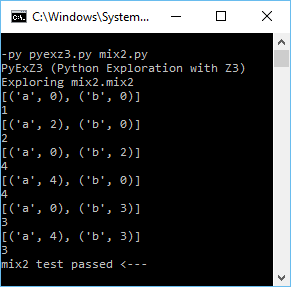
\includegraphics{graphics/PyExZ3-mix2}
	\caption{PyExZ3 produces possible input data for test cases.}
	\label{pic:pyexz3}
\end{figure}
